\section{Durchführung}
\label{sec:Durchführung}

Wie in Kapitel \ref{sec:molwärme} erwähnt wird die Molwärme $C_V$ indirekt über die Messung der spezifische Wärmekapazität $c_\text{k}$ bestimmt.
Diese Messung kann mit einem Kalorimeter wie in Abbildung \ref{fig:abb1} durchgeführt werden.
\begin{figure}
\centering
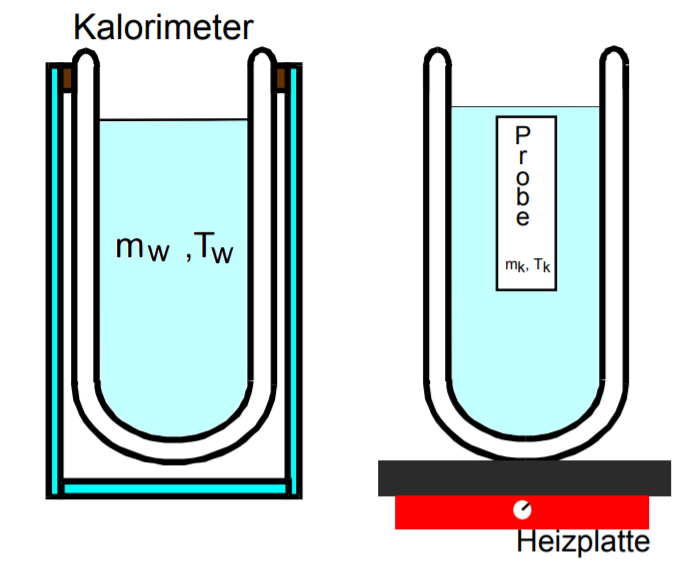
\includegraphics[height=6.0cm]{data/abb1.png}
\caption{Schematischer Aufbau eines Kalorimeters. \cite{V201}}
\label{fig:abb1}
\end{figure}

\subsection{Bestimmung der Wärmekapazität des Kalorimeters}
\label{sec:Durchführung_Kalo}

Die Wärmekapazität des Kalorimeters $c_\text{g} m_\text{g}$ muss bekannt sein, um die spezifische Wärmekapazität eines Materials bestimmen zu können.
Deshalb wird eine zusätliche Messung nur mit Wasser durchgeführt.
Die Massen $m_\text{x}$ und $m_\text{y}$ (zwei ungefähr gleichgroßer Wassermengen) werden bestimmt.
Es sollte ein ähnlich hoher Wasserstand des Kalorimeters erreicht werden wie bei den folgenden Messungen.
Die eine Wassermenge wird in das Kalorimeter gegeben und nach einer kurzen Zeit des Wärmeausgleichs die Temperatur $T_\text{x}$ gemessen.
Die andere Wassermenge wird auf etwa $\SI{90}{\celsius}$ erhitzt und die Temperatur $T_\text{y}$ gemessen.
Anschließend wird das warme Wasser in das Kalorimeter gegeben und nachdem sich ein Gleichgewicht einstellt, die Mischtemperatur $T_\text{m}$ gemessen.

\subsection{Bestimmung der spezifischen Wärmekapazität verschiedener Stoffe}
\label{sec:Durchführung_Stoffe}

Die Messung läuft ähnlich ab wie im vorherigen Abschnitt \ref{sec:Durchführung_Kalo}.
Das Kalorimeter wird mit Wasser befüllt, dessen Masse vorher $m_\text{w}$ bestimmt wird.
Nach kurzer Zeit des Temperaturausgleichs wird die Temperatur des Wassers $T_\text{w}$ gemessen.
Die Materialprobe, deren Wärmekapazität $c_\text{k}$ bestimmt werden soll, wird gewogen und auf etwa \SI{90}{\celsius} erhitzt.
Bevor die erhitzte Probe in das Kalorimeter getaucht wird, wird die Temperatur $T_\text{k}$ gemessen.
Nachdem der Wärmeaustausch zwischen Probe und Wasser abgeschlossen ist, wird die Mischtemperatur $T_\text{m}$ gemessen.
